\chapter[Capítulo 4]{Resultados Obtidos}
\label{ch:cap4}

  Ao final deste trabalho obtivemos a construção de um sistema de design usando a ferramenta Figma. Este SD não só contem os principais elementos usados atualmente na biblioteca de front-end, escrita em Angular, pelo Tribunal de contas do Estado do Rio Grande Do Norte como tambem inclue algumas sugestões de melhoria e evolução para esta biblioteca, permitindo que com algumas alterações a mesma possa manter uma identidade visual mais consistente entre seus sistemas a serem desenvolvidos no futuro e permita aos usuários manter uma experencia mais uniforme ao transitar entre sistemas mantidos ou desenvolvidos pelo TCE-RN.
  
  Alem disso a bibiliteca de componentes é graças ao uso do Figma versionavel dentro da propria ferramenta, permitindo que evoluções na identidade visual não se tornem incompativeis com sistemas existentes em situação legada. O versionamento dessas versões é feito por meio da publicação de alterações em um padrão muito parecido com o utilizado pela ferramente de versionamento de codigo usada pelo tribunal, o GitLab

  O Sistema de Design desenvolvido permite por meio do uso de instâncias de componentes preexistentes sejam criados protótipos de tela de alta fidelidade de maneira rapida e eficiente, permite tambem que os protótipos sejam testados por meio de fluxo de telas associados a ações disparadas por componentes, garantindo durante a fase de levantamento de requisitos usuariso sintam uma experiencia mais proxima da real seja testando um sistema ou uma nova funcionalidade em desenvolvimento.

  Alem disso a biblioteca de componentes pode ser compartilhada publicamente permitindo a qualquer cidadão com interesse de desenvolver alguma funcionalidade ou sistema que consuma dados fornecidos pelo TCE-RN mantenha a mesma conformidade com a identidade visual dos sistemas produzidos pelo Tribuinal de Contas.

  Contudo o sistema carece de testes de uso mais extensivos por parte dos desenvolvedores do TCE-RN não só para assegurar e cobrir eventuais falhas mas tambem para assegurar o treinamento dos desenvolvedores e lideres de projetos no uso de protótipos mas tambem na cultura de prototipação antes do desenvolvimento, de modo a permitir que mudanças em fazes iniciais da construção e testes de sistemas e funcionalidades causem um impacto menor no tempo de produção dos mesmos.

% \lipsum[3-5]
 
% \section{Seção}

% \section{Seção 2}\label{secao2}

% O SHAPE é a sigla em inglês para \textit{Symbolic Hierarchical Automated Reliability and Performance Evaluator}. Veja a \autoref{fig:sharpe}.

% \begin{figure}
% 	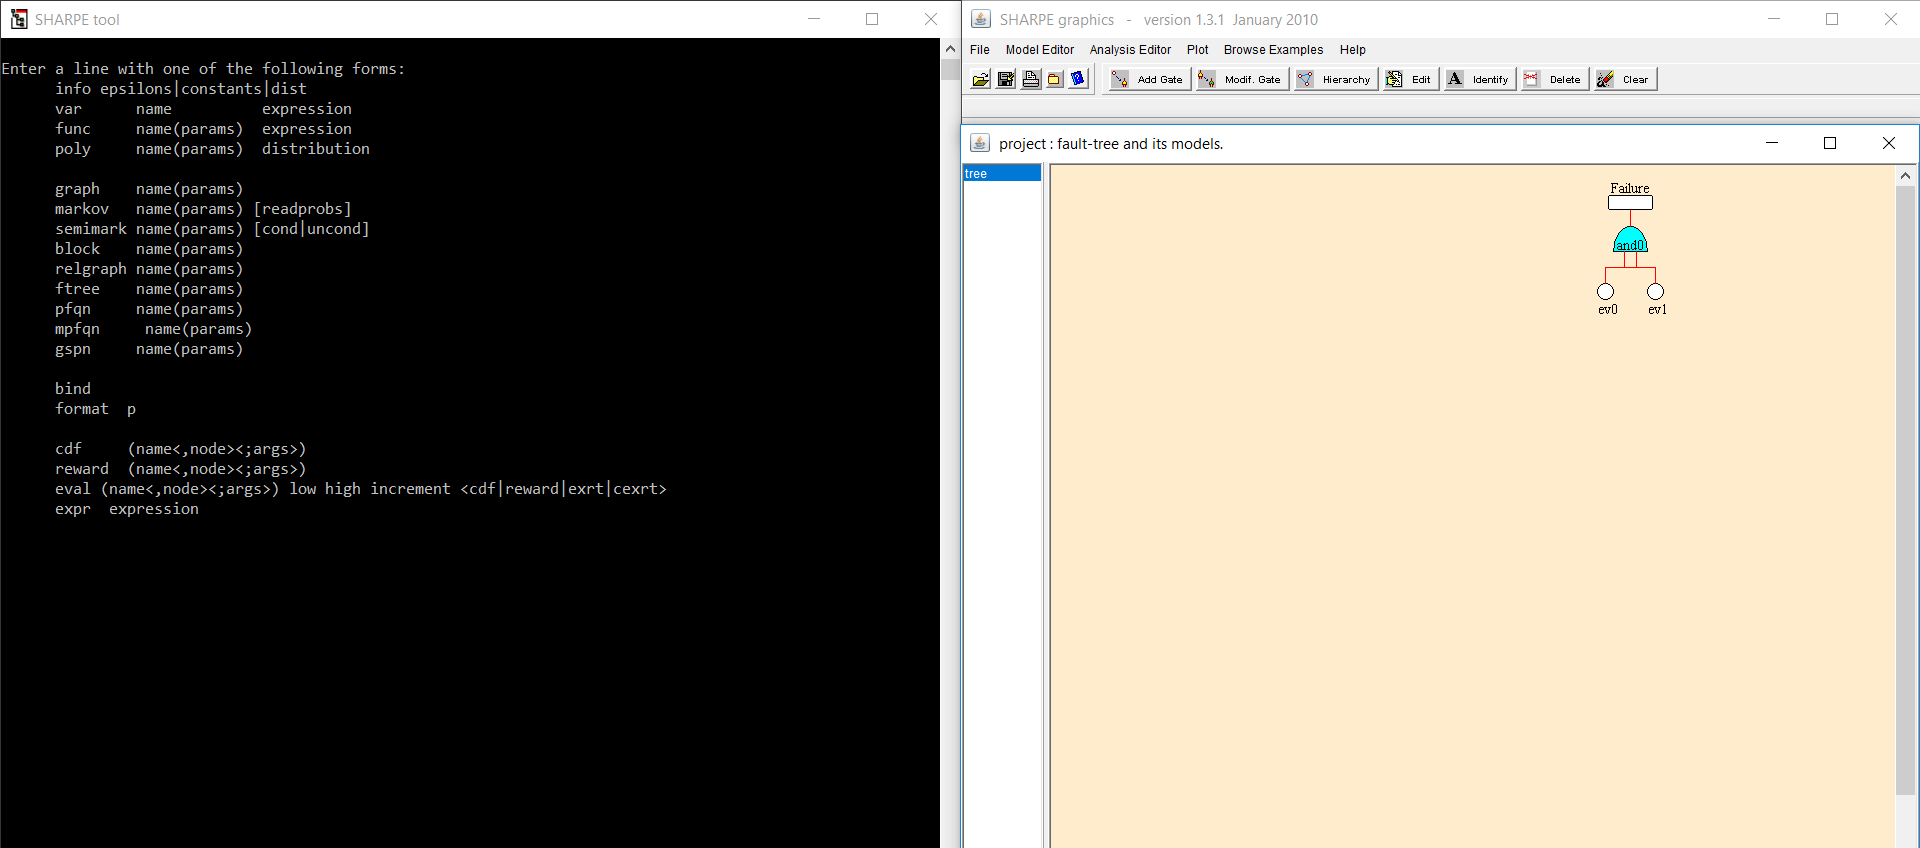
\includegraphics[width=1.0\textwidth, keepaspectratio=true]{sharpe}
% 	\centering
% 	\caption[\textit{Print screen} do SHARPE em linha de comando e em interface gráfica.]{\textit{Print screen} do SHARPE em linha de comando e em interface gráfica.}
% 	\fonte{Elaborada pela autora.}
% 	\label{fig:sharpe}
% \end{figure}